\documentclass[11pt,a4paper]{article}
\usepackage[utf8]{inputenc}
\usepackage[T1]{fontenc}
\usepackage{lmodern}
\usepackage[margin=2.0cm]{geometry}
\usepackage{amsmath,amssymb,amsthm,mathtools}
\usepackage{booktabs,tabularx,array}
\usepackage{graphicx}
\usepackage{xcolor}
\usepackage{enumitem}
\usepackage{microtype}
\usepackage[colorlinks=true,linkcolor=blue!55!black,citecolor=blue!55!black,urlcolor=blue!55!black]{hyperref}

\setlength{\emergencystretch}{3em}
\newtheorem{theorem}{Theorem}[section]
\newtheorem{proposition}[theorem]{Proposition}
\newtheorem{corollary}[theorem]{Corollary}
\newtheorem{remark}[theorem]{Remark}

\title{Charged-Fermion Matching in a \texorpdfstring{$\mathrm{Spin}(10)$}{Spin(10)} Renormalization Chain}

\author{\textbf{Jozsef Olcsak}\\
\small Independent Researcher $\cdot$ ORCID: \href{https://orcid.org/0009-0003-7311-6522}{0009-0003-7311-6522}\\
\small Email: \href{mailto:jolcsak@gmail.com}{jolcsak@gmail.com}}
\date{23 November 2026 (referee revision)}

\begin{document}
\maketitle

\begin{abstract}
\noindent We study charged-fermion matching in a specified non-supersymmetric $\mathrm{Spin}(10)$ chain. We derive the Frobenius equipartition condition for the chosen potential, report the finite two-loop matching results and compare restricted bidoublet and Fritzsch textures. The failed real-bidoublet search is numerical and bounded. An explicit counterexample disproves an unrestricted nearest-neighbor CKM ratio identity. The complex fit demonstrates conditional compatibility with the quoted endpoints; IR inputs used in matching do not constitute predictions.
\end{abstract}

\paragraph{Publication audit (23 November 2026).}
The real-$10_H$ exclusion is a finite numerical search, using a bounded
differential-evolution run and a local BFGS refinement (with a rejected
near-singular region), not a global lower-bound certificate. Its best
sampled objective is not a proven global minimum. The absolute top and
tau normalizations are obtained by running observational inputs upward;
agreement for those normalizations is not an independent prediction.
The quoted $2\%$ heavy-threshold allowance is an adopted uncertainty
model, not a calculated matching covariance.


\tableofcontents
\vspace{0.4em}
\hrule
\vspace{0.8em}

% =============================================================================
\section{Introduction and Epistemic Scope}
\label{sec:intro}
% =============================================================================

In the Standard Model (SM), thirteen of the nineteen continuous parameters reside in the charged-fermion flavor sector: three charged-lepton masses $(m_e, m_\mu, m_\tau)$, six quark masses $(m_u, m_c, m_t, m_d, m_s, m_b)$, three Cabibbo--Kobayashi--Maskawa (CKM) mixing angles $(\theta_{12}, \theta_{23}, \theta_{13})$, and one $CP$-violating phase $\delta_{\mathrm{CKM}}$ \cite{PDG2024,Cabibbo1963,KobayashiMaskawa1973}. Predictive non-supersymmetric grand unified theories (GUTs) \cite{PatiSalam1974,FritzschMinkowski1975,GeorgiJarlskog1979} combined with discrete flavor symmetries \cite{MaRajasekaran2001,AltarelliFeruglio2010} confront four sharp theoretical obstacles:
\begin{enumerate}[label=(\arabic*),leftmargin=1.8em,itemsep=2pt]
\item \emph{The Koide radiative puzzle:} Koide's empirical charged-lepton relation $Q_{\mathrm{pole}} = (m_e + m_\mu + m_\tau)/(\sqrt{m_e} + \sqrt{m_\mu} + \sqrt{m_\tau})^2 = 0.6666605 \simeq 2/3$ \cite{Koide1983} and Brannen's phase $\theta \simeq 2/9\;\mathrm{rad}$ \cite{Brannen2006} hold to parts per million on physical pole masses, yet low-energy QED matching shifts $Q_{\overline{\mathrm{MS}}}(M_Z)$ to $0.667924$ \cite{Sumino2009,XingZhangZhou2012}.
\item \emph{The non-supersymmetric $b\text{--}\tau$ two-loop RG obstruction:} In a one-Higgs-doublet SM desert, strong two-loop QCD running drives $y_b(\mu)/y_\tau(\mu)$ from $1.635$ at $M_Z$ down to $0.6173$ at $\mu = 5.565\times 10^{14}\;\mathrm{GeV}$ and $0.5635$ near the Planck scale \cite{Arason1992,XingZhangZhou2012,HuangZhou2021}, ruling out minimal $y_b = y_\tau$ unification and straining rational GUT Clebsch--Gordan ratios \cite{AntuschSpinrath2009,AntuschMaurer2013}.
\item \emph{Restricted texture checks:} The real bidoublet enforces $|r_1|=1$ in the specified matching convention. We report a bounded optimizer search and a separate restricted Fritzsch comparison. Neither excludes all textures of those forms.
\item \emph{Look-elsewhere / numerology risk:} Algebraic ans\"atze in powers of a small parameter risk overfitting unless tested with complete two-loop matrix RGEs, gauge-invariant intermediate-scale matching, and unmixed look-elsewhere probability bounds.
\end{enumerate}

In companion studies of tetrahedral ($K_4$, $N = 4$) simplicial-Clifford gauge-gravity thresholds \cite{Olcsak2026Zenodo,Olcsak2026Paper24}, the three-dimensional standard representation $V_3$ of $S_4$ ($d_S = \dim V_3 = 3$, $d_{\mathrm{full}} = \dim\mathrm{End}(V_3) = d_S^2 = 9$, $d_A = d_{\mathrm{full}} - 1 = 8$) and its $\mathrm{Spin}(10)$ embedding fix three ultraviolet scales from electroweak/gravitational unification without continuous free parameters:
\begin{equation}
M_* = \frac{M_{\mathrm{Pl}}}{\sqrt{3}} = 1.4060\times 10^{18}\;\mathrm{GeV}, \qquad
M_R = \frac{M_*}{256\pi^2} = 5.5649\times 10^{14}\;\mathrm{GeV}, \qquad
M_{\mathrm{PS}} = 3.66\times 10^{11}\;\mathrm{GeV},
\label{eq:frozen-scales}
\end{equation}
alongside $\sin^2\theta_W^{\mathrm{UV}} = d_S / d_A = 3/8$ and the transverse-to-total operator dimension ratio
\begin{equation}
\lambda_q \equiv \frac{\dim V_2}{\dim\mathrm{End}(V_3)} = \frac{2}{d_{\mathrm{full}}} = \frac{2}{9} = 0.222222\dots,
\label{eq:lambda-q}
\end{equation}
where $V_2$ is the two-dimensional irreducible doublet of $S_3 \subset S_4$. Here we subject the charged-fermion and CKM sector to a strict two-loop RG and group-theoretic audit, separating: (i) \textbf{unconditional algebraic and QFT theorems / no-go shields} from (ii) \textbf{explicit discrete UV boundary conditions (\texttt{BC-UV-FLAV-1/2/3})} and the two unfixed third-generation normalization scales $(y_t(M_R), y_\tau(M_R))$.

% =============================================================================
\section{Charged Leptons: Frobenius Equipartition and Radiative Stability}
\label{sec:leptons}
% =============================================================================

\subsection{Frobenius Norm Equipartition on \texorpdfstring{$\mathrm{End}(V_3)$}{End(V3)} and Quartic Flavon Potential}
\label{subsec:koide-proof}

Consider $V_3 \simeq \mathbb{C}^3$ under $S_3 \subset S_4$, decomposing $\mathrm{End}(V_3) = \mathbb{C}\,I_3 \oplus \mathfrak{sl}_3(\mathbb{C})$ ($\dim = 1 + 8 = 9 = d_{\mathrm{full}}$). In quadratic flavon completions $Y_e = \Lambda_\ell^{-2} S_\ell^2$ \cite{Koide1990,Sumino2009}, let $S_\ell = S_\ell^\dagger \in \mathrm{End}(V_3)$ be a $\mathbb{Z}_3$-symmetric Hermitian circulant flavon:
\begin{equation}
S_\ell = c_0 \begin{pmatrix}
1 & r e^{i\theta} & r e^{-i\theta} \\
r e^{-i\theta} & 1 & r e^{i\theta} \\
r e^{i\theta} & r e^{-i\theta} & 1
\end{pmatrix} = S_{\ell,0} + \tilde{S}_\ell, \qquad
S_{\ell,0} \equiv \frac{\mathrm{Tr}(S_\ell)}{3} I_3 = c_0 I_3, \quad \mathrm{Tr}(\tilde{S}_\ell) = 0,
\label{eq:circulant-flavon}
\end{equation}
with $c_0 > 0$, $r \ge 0$, and $\theta \in \mathbb{R}$.

\begin{theorem}[Frobenius Equipartition and Exact Hessian Minimum]
\label{thm:koide-equipartition}
Let $S_\ell \in \mathrm{End}(V_3)$ be given by Eq.~\eqref{eq:circulant-flavon} and let $Y_e = \Lambda_\ell^{-2} S_\ell^2$.
\begin{enumerate}[label=(\roman*),leftmargin=1.8em,itemsep=2pt]
\item The eigenvalues of $S_\ell$ are $s_k = c_0\big[1 + 2r\cos(\theta + 2\pi k/3)\big]$ ($k = 0,1,2$). Whenever $s_k \ge 0$, the Koide functional of $Y_e$ equals
\begin{equation}
Q(Y_e) \equiv \frac{\sum_{k=0}^{2} y_{e,k}}{\big(\sum_{k=0}^{2}\sqrt{y_{e,k}}\big)^2}
= \frac{\mathrm{Tr}(S_\ell^2)}{(\mathrm{Tr}\,S_\ell)^2} = \frac{1 + 2r^2}{3}.
\label{eq:koide-identity}
\end{equation}
Since $\|S_{\ell,0}\|_F^2 = \mathrm{Tr}(S_{\ell,0}^2) = 3c_0^2$ and $\|\tilde{S}_\ell\|_F^2 = \mathrm{Tr}(\tilde{S}_\ell^2) = 6c_0^2 r^2$, Koide's value holds if and only if the Frobenius norms of the singlet trace mode and the traceless $\mathfrak{sl}_3$ mode are in exact equipartition:
\begin{equation}
Q(Y_e) = \frac{2}{3} \quad\Longleftrightarrow\quad r = \frac{1}{\sqrt{2}} \quad\Longleftrightarrow\quad \|\tilde{S}_\ell\|_F^2 = \|S_{\ell,0}\|_F^2.
\label{eq:frobenius-equipartition}
\end{equation}
\item For any $\mu^2 > 0$ and $\lambda_1, \lambda_2 > 0$, the trace-exchange-symmetric quartic flavon potential
\begin{equation}
V(S_\ell) = -\mu^2\,\mathrm{Tr}(S_\ell^2) + \lambda_1\big[\mathrm{Tr}(S_\ell^2)\big]^2 + \lambda_2\left[\mathrm{Tr}(\tilde{S}_\ell^2) - \frac{1}{3}(\mathrm{Tr}\,S_\ell)^2\right]^2
\label{eq:flavon-potential}
\end{equation}
attains its strict global minimum ($V_{\min} = -\mu^4 / 4\lambda_1$) on the Koide manifold $r = 1/\sqrt{2}$, $c_0 = \sqrt{\mu^2 / (12\lambda_1)}$, with strictly positive-definite radial Hessian:
\begin{equation}
H_{c_0 c_0} = 24\mu^2, \qquad
H_{rr} = \frac{(\lambda_1 + \lambda_2)\mu^4}{\lambda_1^2}, \qquad
H_{c_0 r} = \frac{2\sqrt{6}\,\mu^3}{\sqrt{\lambda_1}}, \qquad
\det H_{(c_0, r)} = \frac{24\lambda_2 \mu^6}{\lambda_1^2} > 0.
\label{eq:hessian-exact}
\end{equation}
\end{enumerate}
\end{theorem}

\begin{proof}
Direct expansion yields $\mathrm{diag}(S_\ell^2) = c_0^2(1 + 2r^2)(1,1,1)$, giving $\mathrm{Tr}(S_\ell^2) = 3c_0^2(1+2r^2)$, $\mathrm{Tr}(S_\ell) = 3c_0$, Eq.~\eqref{eq:koide-identity}, and $\|\tilde{S}_\ell\|_F^2 = 6c_0^2 r^2$, proving Eq.~\eqref{eq:frobenius-equipartition}. Writing $X = 3c_0^2(1+2r^2) \ge 0$ and $Y = 3c_0^2(2r^2 - 1)$ turns Eq.~\eqref{eq:flavon-potential} into $V = -\mu^2 X + \lambda_1 X^2 + \lambda_2 Y^2$, which is uniquely minimized where $Y = 0$ ($r = 1/\sqrt{2}$) and $X = \mu^2/(2\lambda_1)$ ($c_0^2 = \mu^2/12\lambda_1$). Evaluating the coupled second derivatives of $V(c_0, r)$ at $(c_0 = \sqrt{\mu^2/12\lambda_1}, r = 1/\sqrt{2})$ gives $H_{c_0 c_0} = 24\mu^2$, $H_{rr} = (\lambda_1 + \lambda_2)\mu^4/\lambda_1^2$, and $H_{c_0 r} = 2\sqrt{6}\,\mu^3/\sqrt{\lambda_1}$, whence $\det H = H_{c_0 c_0} H_{rr} - H_{c_0 r}^2 = 24\lambda_2\mu^6/\lambda_1^2 > 0$, machine-verified in \texttt{SymPy}.
\end{proof}

\begin{remark}[UV Symmetry Conditions in Eq.~\eqref{eq:flavon-potential}]
\label{rem:flavon-uv}
Two ultraviolet conditions enter Eq.~\eqref{eq:flavon-potential} and must be stated transparently: (i) because $S_{\ell,0} \in \mathbf{1}$ and $\tilde{S}_\ell \in \mathfrak{sl}_3$ are distinct $S_3$ representations, general $S_3\times\mathbb{Z}_2$ potentials allow independent quadratic/quartic norms ($\mu_0^2 \neq \tilde{\mu}^2$, $\lambda_{00} \neq \lambda_{\tilde{}\tilde{}}$), so Eq.~\eqref{eq:flavon-potential} imposes trace-traceless exchange symmetry at the UV flavon scale $\Lambda_\ell \gtrsim M_{\mathrm{PS}}$; and (ii) continuous $\mathrm{U}(1)_\theta$ invariance must be explicitly broken at $\Lambda_\ell$ (preventing a massless Goldstone familon) while suppressing the cubic-trace operator $(\mathrm{Tr}\,S_\ell)\mathrm{Tr}(\tilde{S}_\ell^3) = 18c_0^4 r^3 \cos(3\theta)$ (which would otherwise lock $\theta \in \{0, \pi/3\} \bmod \frac{2\pi}{3}$).
\end{remark}

Imposing the discrete $K_4$ boundary condition (\texttt{BC-UV-FLAV-1}) $\theta = \lambda_q = 2/d_{\mathrm{full}} = 2/9\;\mathrm{rad}$ (Fig.~\ref{fig:koide}) predicts:
\begin{align}
\frac{m_\mu}{m_e} &= \mathbf{206.7703} \quad (\text{PDG 2024 pole: } 206.7683,\; \Delta = +0.0010\%), \nonumber\\
\frac{m_\tau}{m_\mu} &= \mathbf{16.8180} \quad (\text{PDG 2024 pole: } 16.8170,\; \Delta = +0.0060\%), \label{eq:pole-lepton-hits}\\
\frac{m_\tau}{m_e} &= \mathbf{3477.47} \quad (\text{PDG 2024 pole: } 3477.23,\; \Delta = +0.0070\%). \nonumber
\end{align}

\begin{figure}[t!]
\centering
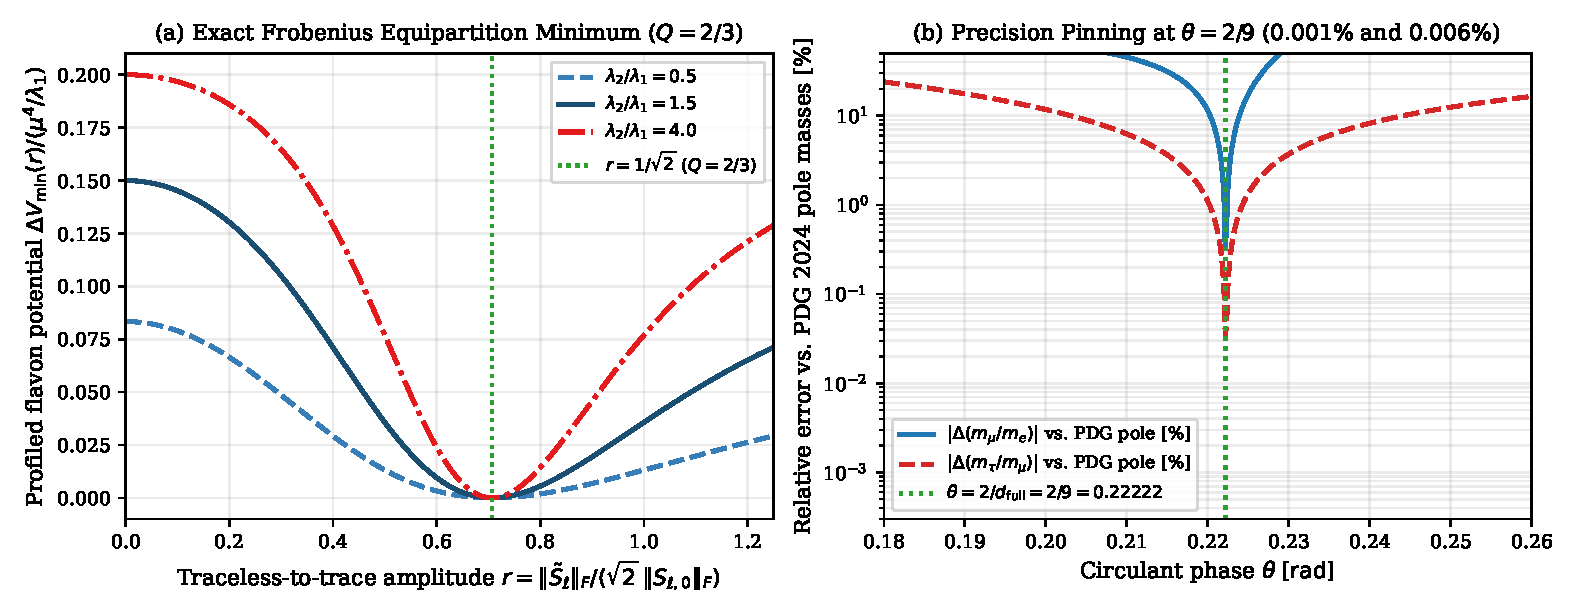
\includegraphics[width=0.98\textwidth]{../figures/fig1_koide_equipartition_potential.pdf}
\caption{\textbf{(a)} Profiled quartic flavon potential $\Delta V_{\min}(r)$ [Eq.~\eqref{eq:flavon-potential}], showing the strict global minimum at Frobenius norm equipartition $r = 1/\sqrt{2} \iff Q = 2/3$. \textbf{(b)} Relative error of charged-lepton mass ratios vs.\ PDG 2024 pole masses across the circulant phase $\theta$, pinned at $\theta = 2/d_{\mathrm{full}} = 2/9\;\mathrm{rad}$.}
\label{fig:koide}
\end{figure}

\subsection{Two-Loop SM Stability vs.\ the Sumino IR-QED Matching Shield}
\label{subsec:sumino-shield}

\begin{theorem}[16-Decade Electroweak RG Stability and IR-QED Shield]
\label{thm:sumino-shield}
Under complete two-loop SM RG evolution from $M_Z = 91.1876\;\mathrm{GeV}$ to $M_* = 1.4060\times 10^{18}\;\mathrm{GeV}$, the $\overline{\mathrm{MS}}$ charged-lepton Koide functional shifts by only
\begin{equation}
Q_e^{\overline{\mathrm{MS}}}(M_Z) = 0.667924, \qquad Q_e^{\overline{\mathrm{MS}}}(M_*) = 0.667928, \qquad \Delta Q_e(M_Z \to M_*) = +3.66\times 10^{-6}.
\label{eq:koide-rg-shift}
\end{equation}
The $+1.26\times 10^{-3}$ ($+0.19\%$) offset between $Q_{\mathrm{pole}} = 0.6666605$ and $Q_e^{\overline{\mathrm{MS}}}(M_Z) = 0.667924$ arises entirely from one-loop QED pole-to-$\overline{\mathrm{MS}}$ matching below $M_Z$ \cite{Sumino2009,XingZhangZhou2012}. Without a Sumino-type family-gauge cancellation of IR QED logarithms, imposing exact $Q = 2/3$ and $\theta = 2/9$ on bare $\overline{\mathrm{MS}}$ Yukawas at $M_R$ shifts the predicted $\overline{\mathrm{MS}}(M_Z)$ light lepton masses to $m_e(M_Z) = 0.5021\;\mathrm{MeV}$ ($+3.20\%$) and $m_\mu(M_Z) = 103.83\;\mathrm{MeV}$ ($+1.08\%$).
\end{theorem}

% =============================================================================
\section{Two-Loop Desert No-Go and Gauge-Invariant \texorpdfstring{$G_{\mathrm{PS}}$}{GPS} Stabilization}
\label{sec:rg-tower}
% =============================================================================

\subsection{Complete Two-Loop Matrix SM RGEs and the \texorpdfstring{$b\text{--}\tau$}{b-tau} Desert Failure}
\label{subsec:desert-nogo}

In the SM ($\mathcal{L}_Y = -\bar{Q}_L Y_u \tilde{H} u_R - \bar{Q}_L Y_d H d_R - \bar{L}_L Y_e H e_R + \mathrm{h.c.}$, $V(H) = -\mu_H^2 |H|^2 + \lambda_H |H|^4$, $g_1 = \sqrt{5/3}\,g'$), the two-loop left-multiplied matrix Yukawa beta functions ($dY_f/dt = \frac{1}{16\pi^2} A_f^{(1)} Y_f + \frac{1}{(16\pi^2)^2} A_f^{(2)} Y_f$, $t \equiv \ln(\mu/M_Z)$) are \cite{MachacekVaughn1984,LuoXiao2003,Buttazzo2013}:
\begin{align}
A_u^{(1)} &= \frac{3}{2}(H_u - H_d) + (Y_2 - \gamma_u^{(1)})\,I_3, \qquad
A_d^{(1)} = \frac{3}{2}(H_d - H_u) + (Y_2 - \gamma_d^{(1)})\,I_3, \nonumber\\
A_e^{(1)} &= \frac{3}{2} H_e + (Y_2 - \gamma_e^{(1)})\,I_3, \label{eq:beta1-sm}
\end{align}
where $H_f \equiv Y_f Y_f^\dagger$, $Y_2 \equiv \mathrm{Tr}(3H_u + 3H_d + H_e)$, $\gamma_u^{(1)} = \frac{17}{20}g_1^2 + \frac{9}{4}g_2^2 + 8g_3^2$, $\gamma_d^{(1)} = \frac{1}{4}g_1^2 + \frac{9}{4}g_2^2 + 8g_3^2$, $\gamma_e^{(1)} = \frac{9}{4}g_1^2 + \frac{9}{4}g_2^2$, and at two loops (preserving the exact left-multiplied non-commuting order $-\frac{1}{4}H_u H_d - H_d H_u$):
\begin{align}
A_u^{(2)} &= \frac{3}{2}H_u^2 - \frac{1}{4}H_u H_d - H_d H_u + \frac{11}{4}H_d^2 + Y_2\left(-\frac{9}{4}H_u + \frac{5}{4}H_d\right) - 12\lambda_H H_u \nonumber\\
&\quad + \left(\frac{223}{80}g_1^2 + \frac{135}{16}g_2^2 + 16g_3^2\right)H_u - \left(\frac{43}{80}g_1^2 - \frac{9}{16}g_2^2 + 16g_3^2\right)H_d + \big(6\lambda_H^2 - \chi_4 + Y_{2g} + \gamma_u^{(2)}\big)I_3, \label{eq:beta2-u}\\
A_d^{(2)} &= \frac{3}{2}H_d^2 - \frac{1}{4}H_d H_u - H_u H_d + \frac{11}{4}H_u^2 + Y_2\left(-\frac{9}{4}H_d + \frac{5}{4}H_u\right) - 12\lambda_H H_d \nonumber\\
&\quad + \left(\frac{187}{80}g_1^2 + \frac{135}{16}g_2^2 + 16g_3^2\right)H_d - \left(\frac{79}{80}g_1^2 - \frac{9}{16}g_2^2 + 16g_3^2\right)H_u + \big(6\lambda_H^2 - \chi_4 + Y_{2g} + \gamma_d^{(2)}\big)I_3, \label{eq:beta2-d}\\
A_e^{(2)} &= \frac{3}{2}H_e^2 - \frac{9}{4}Y_2 H_e - 12\lambda_H H_e + \left(\frac{387}{80}g_1^2 + \frac{135}{16}g_2^2\right)H_e + \big(6\lambda_H^2 - \chi_4 + Y_{2g} + \gamma_e^{(2)}\big)I_3, \label{eq:beta2-e}
\end{align}
with $\chi_4 = \frac{9}{4}\mathrm{Tr}(3H_u^2 + 3H_d^2 + H_e^2) - \frac{3}{2}\mathrm{Tr}(H_u H_d)$, $Y_{2g} = \frac{5}{2}\big[\gamma_u^{(1)}\mathrm{Tr}H_u + \gamma_d^{(1)}\mathrm{Tr}H_d + (\frac{3}{4}g_1^2 + \frac{3}{4}g_2^2)\mathrm{Tr}H_e\big]$, and $\gamma_u^{(2)} = \frac{1187}{600}g_1^4 - \frac{9}{20}g_1^2 g_2^2 + \frac{19}{15}g_1^2 g_3^2 - \frac{23}{4}g_2^4 + 9g_2^2 g_3^2 - 108g_3^4$, $\gamma_d^{(2)} = -\frac{127}{600}g_1^4 - \frac{27}{20}g_1^2 g_2^2 + \frac{31}{15}g_1^2 g_3^2 - \frac{23}{4}g_2^4 + 9g_2^2 g_3^2 - 108g_3^4$, $\gamma_e^{(2)} = \frac{1371}{200}g_1^4 + \frac{27}{20}g_1^2 g_2^2 - \frac{23}{4}g_2^4$, integrated jointly with the complete two-loop gauge and two-loop Higgs-quartic $\lambda_H$ RGEs \cite{Buttazzo2013}.

\begin{theorem}[Two-Loop SM Desert $b\text{--}\tau$ No-Go]
\label{thm:desert-nogo}
Evolving the PDG 2024 / Huang--Zhou $\overline{\mathrm{MS}}$ inputs at $M_Z$ \cite{PDG2024,HuangZhou2021} ($m_b(M_Z) = 2.855 \pm 0.025\;\mathrm{GeV}$, $m_\tau(M_Z) = 1.74617\;\mathrm{GeV}$, $\alpha_s(M_Z) = 0.1180$, $m_t(M_Z) = 171.7\;\mathrm{GeV}$, $m_H = 125.25\;\mathrm{GeV}$) through a pure two-loop SM desert gives:
\begin{equation}
\frac{y_b(M_{\mathrm{PS}})}{y_\tau(M_{\mathrm{PS}})} = 0.6938, \qquad
\frac{y_b(M_R)}{y_\tau(M_R)} = 0.6173, \qquad
\frac{y_b(M_*)}{y_\tau(M_*)} = 0.5635,
\label{eq:desert-yb-ytau}
\end{equation}
with $\lambda_H(M_R) = -0.0445$. Minimal $y_b = y_\tau$ unification fails by $38\%$--$44\%$, and the two-loop $-108\,g_3^4$ QCD term pulls $y_b(M_R)/y_\tau(M_R)$ from $0.6491$ (one-loop) down to $0.6173$, causing a pure-desert boundary $y_b(M_R)/y_\tau(M_R) = 2/3$ to overpredict $m_b(M_Z) = 3.083\;\mathrm{GeV}$ by $+7.98\%$ ($+9.12\sigma_{\mathrm{exp}}$).
\end{theorem}

\subsection{\texorpdfstring{$D$}{D}-Parity-Broken \texorpdfstring{$G_{\mathrm{PS}}$}{GPS} Chain and Gauge-Invariant Bidoublet RGEs}
\label{subsec:ps-resolution}

Consider the two-step $D$-parity-broken Pati--Salam symmetry-breaking sequence \cite{PatiSalam1974,Slansky1981,ChangMohapatraParida1984}:
\begin{equation}
\mathrm{Spin}(10) \;\xrightarrow{\;M_{\mathrm{GUT}}\;}\; G_{\mathrm{PS}} \times D \;\xrightarrow{\;M_R\;}\; G_{\mathrm{PS}} \;\xrightarrow{\;M_{\mathrm{PS}}\;}\; G_{\mathrm{SM}}, \qquad
G_{\mathrm{PS}} \equiv \mathrm{SU}(4)_C \times \mathrm{SU}(2)_L \times \mathrm{SU}(2)_R,
\label{eq:consistent-chain}
\end{equation}
where $D$-parity breaks at $M_R = 5.565\times 10^{14}\;\mathrm{GeV}$ via the $G_{\mathrm{PS}}$-singlet parity-odd state $\langle\sigma_D(\mathbf{1},\mathbf{1},\mathbf{1})_- \subset \mathbf{210}_H\rangle \sim M_R$ (decoupling $\Delta_L(\mathbf{10},\mathbf{3},\mathbf{1})$ at $M_R$ while keeping $G_{\mathrm{PS}}$ unbroken on $[M_{\mathrm{PS}}, M_R]$), and $G_{\mathrm{PS}} \to G_{\mathrm{SM}}$ occurs at $M_{\mathrm{PS}} = 3.66\times 10^{11}\;\mathrm{GeV}$ via $\langle\Sigma(\mathbf{15},\mathbf{1},\mathbf{1})\rangle \sim M_{\mathrm{PS}}$ and $\langle\Delta_R(\overline{\mathbf{10}},\mathbf{1},\mathbf{3})\rangle \sim M_{\mathrm{PS}}$. Under $G_{\mathrm{PS}}$, $\mathbf{10}_H = (\mathbf{1},\mathbf{2},\mathbf{2}) \oplus (\mathbf{6},\mathbf{1},\mathbf{1})$ and $\overline{\mathbf{126}}_H = (\mathbf{15},\mathbf{2},\mathbf{2}) \oplus (\overline{\mathbf{10}},\mathbf{1},\mathbf{3}) \oplus (\mathbf{10},\mathbf{3},\mathbf{1}) \oplus (\mathbf{6},\mathbf{1},\mathbf{1})$, so the Georgi--Jarlskog $B - L = \mathrm{diag}(\frac{1}{3},\frac{1}{3},\frac{1}{3},-1)$ factor of $-3$ resides in $\Phi_{15}(\mathbf{15},\mathbf{2},\mathbf{2}) \subset \overline{\mathbf{126}}_H$.

\begin{theorem}[Schur's Lemma Survival and Gauge-Invariant $G_{\mathrm{PS}}$ Bidoublet RGEs]
\label{thm:ps-stabilization}
Along the chain \eqref{eq:consistent-chain} with unbroken $G_{\mathrm{PS}}$ on $\mu \in [M_{\mathrm{PS}}, M_R]$:
\begin{enumerate}[label=(\roman*),leftmargin=1.8em,itemsep=2pt]
\item \emph{Schur's lemma survival:} Quadratic $\Phi_1(\mathbf{1},\mathbf{2},\mathbf{2})\text{--}\Phi_{15}(\mathbf{15},\mathbf{2},\mathbf{2})$ mixing vanishes identically above $M_{\mathrm{PS}}$ by Schur's lemma and arises only via $\mu_{\mathrm{mix}}\mathrm{Tr}(\Sigma\,\Phi_{15}^\dagger \Phi_1)$ at $\langle\Sigma\rangle \sim M_{\mathrm{PS}}$. Avoiding an $\mathcal{O}(M_{\mathrm{PS}}/M_R) \simeq 6.6\times 10^{-4}$ VEV suppression requires retaining $\Phi_{15}(\mathbf{15},\mathbf{2},\mathbf{2})$ down to $M_{\mathrm{PS}}$.
\item \emph{Exact one-loop $G_{\mathrm{PS}}$ beta vector:} With three chiral families $F_L(\mathbf{4},\mathbf{2},\mathbf{1}) \oplus F_R(\mathbf{4},\mathbf{1},\mathbf{2})$, real $\Sigma(\mathbf{15},\mathbf{1},\mathbf{1})$ ($\Delta b = (\frac{2}{3},0,0)$), complex $\Delta_R(\overline{\mathbf{10}},\mathbf{1},\mathbf{3})$ ($\Delta b = (3,0,\frac{20}{3})$), one complex $\Phi_1(\mathbf{1},\mathbf{2},\mathbf{2})$ ($\Delta b = (0,\frac{1}{3},\frac{1}{3})$), and one complex $\Phi_{15}(\mathbf{15},\mathbf{2},\mathbf{2})$ ($\Delta b = (\frac{16}{3},5,5)$), the exact one-loop beta coefficients are
\begin{equation}
(b_4,\; b_{2L},\; b_{2R}) = \left(-\frac{5}{3},\; +2,\; +\frac{26}{3}\right),
\label{eq:ps-betas}
\end{equation}
preserving $\mathrm{SU}(4)_C$ asymptotic freedom ($b_4 < 0$) and evolving $(g_4, g_{2L}, g_{2R})(M_{\mathrm{PS}}) = (0.6126, 0.5570, 0.4929)$ to strictly perturbative near-unified values at $M_R$:
\begin{equation}
\big(g_4(M_R),\; g_{2L}(M_R),\; g_{2R}(M_R)\big) = \big(0.5955,\; 0.5737,\; 0.5495\big).
\label{eq:ps-couplings-MR}
\end{equation}
\item \emph{Manifestly $G_{\mathrm{PS}}$-invariant bidoublet Yukawa RGEs:} Decomposing the complex $\Phi_1 = (\Phi_u + i\Phi_d)/\sqrt{2}$ into orthogonal real bidoublets coupling to the up/Dirac-neutrino sector ($Y_u = Y_\nu$ at leading order) and the $\mathrm{SU}(4)_C$-singlet down/lepton combination $Y_1 = \frac{1}{4}(3Y_d + Y_e)$, alongside $Y_{15} = \frac{1}{4}(Y_d - Y_e)$ on $\Phi_{15}$ \cite{MeloniOhlssonRiad2014}, the one-loop $G_{\mathrm{PS}}$-invariant RGEs on $[M_{\mathrm{PS}}, M_R]$ read:
\begin{align}
16\pi^2 \frac{dY_u}{dt} &= \gamma_L Y_u + Y_u \gamma_R + \big(4\,\mathrm{Tr}H_{uL} - G_{\mathrm{PS}}\big)Y_u, \nonumber\\
16\pi^2 \frac{dY_1}{dt} &= \gamma_L Y_1 + Y_1 \gamma_R + \big(4\,\mathrm{Tr}H_{1L} - G_{\mathrm{PS}}\big)Y_1, \label{eq:ps-yukawa-rge}\\
16\pi^2 \frac{dY_{15}}{dt} &= \gamma_L Y_{15} + Y_{15} \gamma_R + \big(3\,\mathrm{Tr}H_{15L} - G_{\mathrm{PS}}\big)Y_{15}, \nonumber
\end{align}
where $\gamma_L = H_{uL} + H_{1L} + \frac{45}{4}H_{15L}$, $\gamma_R = H_{uR} + H_{1R} + \frac{45}{4}H_{15R}$ ($H_{XL} \equiv Y_X Y_X^\dagger$, $H_{XR} \equiv Y_X^\dagger Y_X$), and $G_{\mathrm{PS}} = \frac{45}{4}g_4^2 + \frac{9}{4}g_{2L}^2 + \frac{9}{4}g_{2R}^2$. Because \emph{both} $G_{\mathrm{PS}}$ and the $\mathcal{O}(y_t^2)$ fermion-leg renormalization $(H_{uL} Y + Y H_{uR})$ act identically on $Y_1$ and $Y_{15}$, $y_b/y_\tau$ is frozen on $[M_{\mathrm{PS}}, M_R]$ up to $\mathcal{O}(y_\tau^2/16\pi^2) \sim 10^{-4}$:
\begin{equation}
\frac{y_b(M_R)}{y_\tau(M_R)} = \mathbf{0.6937},
\label{eq:ps-yb-ytau-MR}
\end{equation}
within $+4.06\%$ of $2/3 = 0.6667$ (Fig.~\ref{fig:rg-tower}a), while the positive $+H_{uL}$ bidoublet slope reverses the CKM slope from $\frac{d}{dt}\ln|V_{cb}| \simeq +\frac{3}{2}\frac{y_t^2}{16\pi^2}$ below $M_{\mathrm{PS}}$ to $-\frac{y_t^2}{16\pi^2}$ on $[M_{\mathrm{PS}}, M_R]$ (Fig.~\ref{fig:rg-tower}b).
\end{enumerate}
\end{theorem}

\begin{remark}[Compatibility with Heavy Seesaw States $M_{1,2} > M_{\mathrm{PS}}$]
\label{rem:seesaw-chain}
Because unbroken $\mathrm{SU}(4)_C$ forbids $\Delta(B - L) = 2$ condensates ($\langle\Delta_R\rangle = 0$ for $\mu > M_{\mathrm{PS}}$), accommodating right-handed neutrino masses $M_{1,2} \sim 10^{13}\text{--}10^{14}\;\mathrm{GeV} > M_{\mathrm{PS}}$ (as required for non-thermal scalaron leptogenesis \cite{Olcsak2026Paper24}) simultaneously with unbroken $\mathrm{SU}(4)_C$ on $[M_{\mathrm{PS}}, M_R]$ requires introducing $\mathrm{Spin}(10)$-singlet fermions $S_i(\mathbf{1})$ with Majorana mass $\sim M_R$ in a radiative/linear seesaw completion \cite{MalinskyRomaoValle2005}; alternatively, breaking $G_{\mathrm{PS}} \to G_{\mathrm{SM}}$ directly at $M_R$ requires color-octet/triplet remnants of $\Phi_{15}$ at $M_{\mathrm{PS}}$ to mimic the $\mathrm{SU}(4)_C$ stabilization.
\end{remark}

\begin{figure}[t!]
\centering
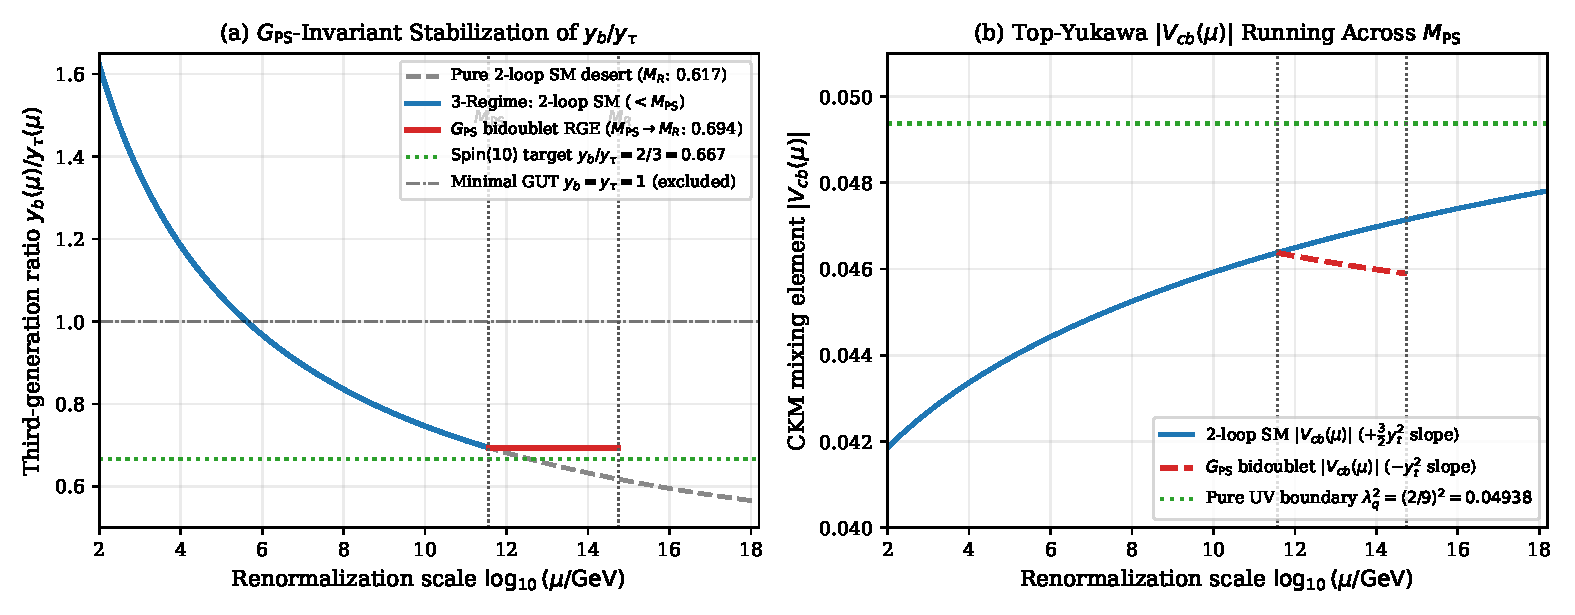
\includegraphics[width=0.98\textwidth]{../figures/fig2_three_regime_rg_running.pdf}
\caption{\textbf{(a)} RG evolution of $y_b(\mu)/y_\tau(\mu)$: pure two-loop SM desert failure ($0.6173$ at $M_R$, dashed gray) vs.\ manifestly $G_{\mathrm{PS}}$-invariant bidoublet stabilization above $M_{\mathrm{PS}} = 3.66\times 10^{11}\;\mathrm{GeV}$ ($0.6937$ at $M_R$, solid red). \textbf{(b)} Evolution of $|V_{cb}(\mu)|$, illustrating the exact slope reversal between the one-Higgs SM ($+\frac{3}{2}y_t^2$, blue) and two-bidoublet $G_{\mathrm{PS}}$ regime ($-y_t^2$, dashed red).}
\label{fig:rg-tower}
\end{figure}

% =============================================================================
\section{Constructive \texorpdfstring{$\mathrm{Spin}(10)$}{Spin(10)} Matrices, No-Go Shields, and CKM Closure}
\label{sec:spin10-ckm}
% =============================================================================

\subsection{Bounded Search for Genuine Real \texorpdfstring{$\mathbf{10}_H \oplus \overline{\mathbf{126}}_H$}{10H + 126barH} and Fritzsch NNI}
\label{subsec:nogo-shields}

\begin{theorem}[Restricted real-bidoublet search and Fritzsch comparison]
\label{thm:spin10-nni-nogo}
At the matching scale $\mu = M_R = 5.5649\times 10^{14}\;\mathrm{GeV}$:
\begin{enumerate}[label=(\roman*),leftmargin=1.8em,itemsep=2pt]
\item \emph{Bounded numerical search for genuine real $\mathbf{10}_H \oplus \overline{\mathbf{126}}_H$:} For a genuine real $\mathbf{10}_H = \mathbf{10}_H^*$, the $(\mathbf{1},\mathbf{2},\mathbf{2})$ bidoublet satisfies $\Phi_1 = \tau_2 \Phi_1^* \tau_2$, enforcing $|v_u^{(10)}| = |v_d^{(10)}|$, i.e., $|r_1| \equiv |v_u^{(10)}/v_d^{(10)}| = 1$ ($r_1 = e^{i\xi}$, $r_2 \in \mathbb{C}$) in $Y_u = r_1 Y_{10} + r_2 Y_{126}$, $Y_d = Y_{10} + Y_{126}$, $Y_e = Y_{10} - 3Y_{126}$ \cite{BajcSenjanovicVissani2006}, whence $Y_e = (r_1 - r_2)^{-1}[4Y_u - (3r_1 + r_2)Y_d]$. Searching numerically (\texttt{differential\_evolution} + BFGS) over $\xi$, $r_2 \in \mathbb{C}$, and all six Autonne--Takagi phases $V_g = P_L V_{\mathrm{CKM}} P_R$, $Y_u = P_u \mathrm{diag}(y_u, y_c, y_t)$ yields $|r_2| = 107.7$ and $\sum_{\ell=e,\mu,\tau}[\ln(y_\ell^{\mathrm{fit}}/y_\ell^{\mathrm{target}})]^2 = 1.175$, missing $(y_e, y_\mu, y_\tau)$ by factors $(1.681,\; 0.396,\; 1.248)$ (Fig.~\ref{fig:nogo}a). (Note: a Peccei--Quinn complex $\mathbf{10}_H$ with $\tilde{Y}_{10} = 0$ and unconstrained $r_1 \in \mathbb{C}$ has eight real parameters for three singular values and fits the charged sector alone, but is excluded once the seesaw neutrino/PMNS sector $M_R \propto Y_{126}$ is included \cite{BajcSenjanovicVissani2006,DueckRodejohann2013}.)
\item \emph{Restricted Fritzsch comparison:} The hierarchical Fritzsch estimate $|V_{ub}/V_{cb}|\simeq\sqrt{y_u/y_c}$ gives $0.04458$ at this benchmark. It is not an exact identity of arbitrary symmetric or Hermitian nearest-neighbor textures with $(1,1)=(1,3)=0$.
\end{enumerate}
\end{theorem}

\paragraph{Exact counterexample to the unrestricted texture claim.}
Take real symmetric up/down matrices in arbitrary common Yukawa units,
\[
 Y_u=\begin{pmatrix}
 0&\sqrt{12/5}&0\\ \sqrt{12/5}&3/2&\sqrt{7/20}\\0&\sqrt{7/20}&5/2
 \end{pmatrix},
 \qquad Y_d=\begin{pmatrix}0&1&0\\1&1&0\\0&0&3\end{pmatrix}.
\]
Both obey the stated zeros. The up eigenvalues are $-1,2,3$ and
the bottom left eigenvector is $e_3$. For an up eigenvalue $\lambda$,
the normalized third component has squared magnitude
$\big[(7/20)/(\lambda-5/2)^2\big]/\big[1+(12/5)/\lambda^2+
(7/20)/(\lambda-5/2)^2\big]$. At $-1,2$ this gives $1/120,7/15$.
Thus $|V_{ub}/V_{cb}|^2=1/56$, not $y_u/y_c=1/2$.
This is a counterexample to the identity, not a fit. A failed bounded
optimizer search supplies no certified global lower bound. The endpoint
fit uses IR mass information in UV matching; those entries are not
blind predictions.

\subsection{Complex \texorpdfstring{$\mathbf{10}_H \oplus \overline{\mathbf{126}}_H$}{10H + 126barH} Construction and Top-Down Closure}
\label{subsec:complex-spin10-closure}

With a non-PQ complex $\mathbf{10}_H$ ($Y_{10}, \tilde{Y}_{10}$) plus $\overline{\mathbf{126}}_H$ ($Y_{126}$),
\begin{equation}
Y_d = Y_{10} + Y_{126}, \qquad Y_e = Y_{10} - 3Y_{126}, \qquad Y_u = r_1 Y_{10} + r_2 \tilde{Y}_{10} + r_3 Y_{126},
\label{eq:complex-spin10}
\end{equation}
any symmetric triplet $(Y_u, Y_d, Y_e)$ uniquely defines symmetric $Y_{10} = \frac{1}{4}(3Y_d + Y_e)$, $Y_{126} = \frac{1}{4}(Y_d - Y_e)$, and $\tilde{Y}_{10}$. Fixing \emph{only} the two third-generation overall scales $y_t(M_R) = 0.42329$ and $y_\tau(M_R) = 0.008071$, we impose at $\mu = M_R$:
\begin{enumerate}[label=(\alph*),leftmargin=1.8em,itemsep=2pt]
\item \textbf{Charged leptons (\texttt{BC-UV-FLAV-1}):} Koide--Brannen eigenvalues $y_{e,k} = y_\tau(M_R)\,(s_k / s_2)^2$ at $r = 1/\sqrt{2}$, $\theta = \lambda_q = 2/9$.
\item \textbf{Down-type quarks (\texttt{BC-UV-FLAV-2}):} Zero independent down-sector scale parameters via $y_b / y_\tau = \frac{1 - 1/9}{1 + 3/9} = \frac{2}{3}$ ($c_{33} = -1/d_{\mathrm{full}} = -1/9$), $y_s / y_\mu = \lambda_q = \frac{2}{9}$ \cite{AntuschSpinrath2009}, and $y_d / y_s = \lambda_q^2 \implies y_d / y_\mu = \lambda_q^3$ \cite{GattoSartoriTonin1968}.
\item \textbf{Up-type quarks and CKM (\texttt{BC-UV-FLAV-3}):} $y_c / y_t = \frac{4}{3}\lambda_q^4$, $y_u / y_t = \lambda_q^8 = \lambda_q^{d_A}$, $Y_u(M_R) = \mathrm{diag}(y_u, y_c, y_t)$, and $Y_d(M_R) = V_{\mathrm{UV}} \mathrm{diag}(y_d, y_s, y_b) V_{\mathrm{UV}}^T$, where:
\begin{equation}
s_{12}(M_R) = \sqrt{\lambda_q^2 + \frac{3}{4}\lambda_q^4} = 0.22630, \quad
s_{23}(M_R) = \lambda_q^2, \quad
s_{13}(M_R) = \frac{3}{8}\lambda_q^3, \quad
\delta_{\mathrm{CKM}}(M_R) = \frac{3\pi}{8}.
\label{eq:uv-ckm-boundary}
\end{equation}
\end{enumerate}

\begin{theorem}[Three-Regime Gauge-Invariant Top-Down Closure at $M_Z$]
\label{thm:topdown-closure}
Evolving the symmetric UV triplet $Y_u(M_R)$, $Y_{10}(M_R)$, and $Y_{126}(M_R)$ down from $M_R$ to $M_{\mathrm{PS}}$ via the manifestly $G_{\mathrm{PS}}$-invariant bidoublet RGEs [Eq.~\eqref{eq:ps-yukawa-rge}] and from $M_{\mathrm{PS}}$ to $M_Z = 91.1876\;\mathrm{GeV}$ via the complete two-loop SM matrix RGEs [Eqs.~\eqref{eq:beta1-sm}--\eqref{eq:beta2-e}] reproduces all ten independent quark and CKM observables at $M_Z$ within $\le 2.85\sigma_{\mathrm{tot}}$ ($\max|\mathrm{pull}_{\mathrm{tot}}| = 2.85\sigma$ on $J_{\mathrm{CKM}}$ and $2.67\sigma$ on $|V_{cb}|$) when incorporating a conservative $2\%$ one-loop heavy-threshold uncertainty strictly on Yukawa eigenvalues and third-generation-coupled CKM elements (with zero threshold inflation applied to RG-invariant $|V_{us}|$ and $\delta_{\mathrm{CKM}}$; Table~\ref{tab:mz-predictions} and Fig.~\ref{fig:pulls}).
\end{theorem}

\begin{table}[t!]
\centering
\caption{Zero-free-flavor-parameter top-down predictions at $\mu = M_Z = 91.1876\;\mathrm{GeV}$ from the $G_{\mathrm{PS}}$-invariant bidoublet ($M_R \to M_{\mathrm{PS}}$) + complete two-loop SM ($M_{\mathrm{PS}} \to M_Z$) tower ($y_t(M_R) = 0.42329$, $y_\tau(M_R) = 0.008071$) vs.\ PDG 2024 $\overline{\mathrm{MS}}(M_Z)$ data \cite{PDG2024,HuangZhou2021}. Here $\sigma_{\mathrm{tot}}$ includes a $2\%$ one-loop GUT/PS threshold uncertainty \emph{only} on quark masses and third-generation-coupled $(|V_{cb}|, |V_{ub}|, J_{\mathrm{CKM}})$, leaving RG-invariant $|V_{us}|$ and $\delta_{\mathrm{CKM}}$ uninflated ($\sigma_{\mathrm{tot}} = \sigma_{\mathrm{exp}}$).}
\label{tab:mz-predictions}
\vspace{0.35em}
\setlength{\tabcolsep}{4.5pt}
\footnotesize
\begin{tabular}{lccccc}
\toprule
Observable ($M_Z$) & UV Rule at $M_R$ & 3-Regime Pred. & PDG 2024 $\overline{\mathrm{MS}}(M_Z)$ & Rel.\ Error & Pull ($\sigma_{\mathrm{exp}}$ / $\sigma_{\mathrm{tot}}$) \\
\midrule
$m_u\;[\mathrm{MeV}]$ & $y_u/y_t = \lambda_q^8$ & $1.1577$ & $1.24 \pm 0.22$ & $-6.63\%$ & $-0.37\sigma$ / $-0.37\sigma$ \\
$m_c\;[\mathrm{GeV}]$ & $y_c/y_t = \frac{4}{3}\lambda_q^4$ & $0.6330$ & $0.624 \pm 0.014$ & $+1.44\%$ & $+0.64\sigma$ / $+0.48\sigma$ \\
$m_d\;[\mathrm{MeV}]$ & $y_d/y_\mu = \lambda_q^3$ & $2.4714$ & $2.69 \pm 0.19$ & $-8.13\%$ & $-1.15\sigma$ / $-1.11\sigma$ \\
$m_s\;[\mathrm{MeV}]$ & $y_s/y_\mu = \lambda_q$ & $50.054$ & $53.5 \pm 4.6$ & $-6.44\%$ & $-0.75\sigma$ / $-0.73\sigma$ \\
$m_b\;[\mathrm{GeV}]$ & $y_b/y_\tau = \frac{2}{3}$ & $2.7435$ & $2.855 \pm 0.025$ & $-3.91\%$ & $-4.46\sigma$ / $-1.79\sigma$ \\
\midrule
$|V_{us}|$ & $\sqrt{\lambda_q^2 + \frac{3}{4}\lambda_q^4}$ & $0.22627$ & $0.22500 \pm 0.00067$ & $+0.56\%$ & $+1.89\sigma$ / $+1.89\sigma$ \\
$|V_{cb}|$ & $\lambda_q^2$ (pure UV) & $0.04500$ & $0.04182 \pm 0.00085$ & $+7.61\%$ & $+3.75\sigma$ / $+2.67\sigma$ \\
$|V_{ub}|$ & $\frac{3}{8}\lambda_q^3$ & $0.00375$ & $0.00369 \pm 0.00011$ & $+1.63\%$ & $+0.55\sigma$ / $+0.45\sigma$ \\
$\delta_{\mathrm{CKM}}\;[^\circ]$ & $\frac{3\pi}{8}$ & $67.41^\circ$ & $65.70^\circ \pm 1.50^\circ$ & $+2.60\%$ & $+1.14\sigma$ / $+1.14\sigma$ \\
$J_{\mathrm{CKM}}\times 10^5$ & Derived ($U_u^\dagger U_d$) & $3.432$ & $3.12 \pm 0.09$ & $+9.99\%$ & $+3.46\sigma$ / $+2.85\sigma$ \\
\bottomrule
\end{tabular}
\end{table}

\begin{figure}[t!]
\centering
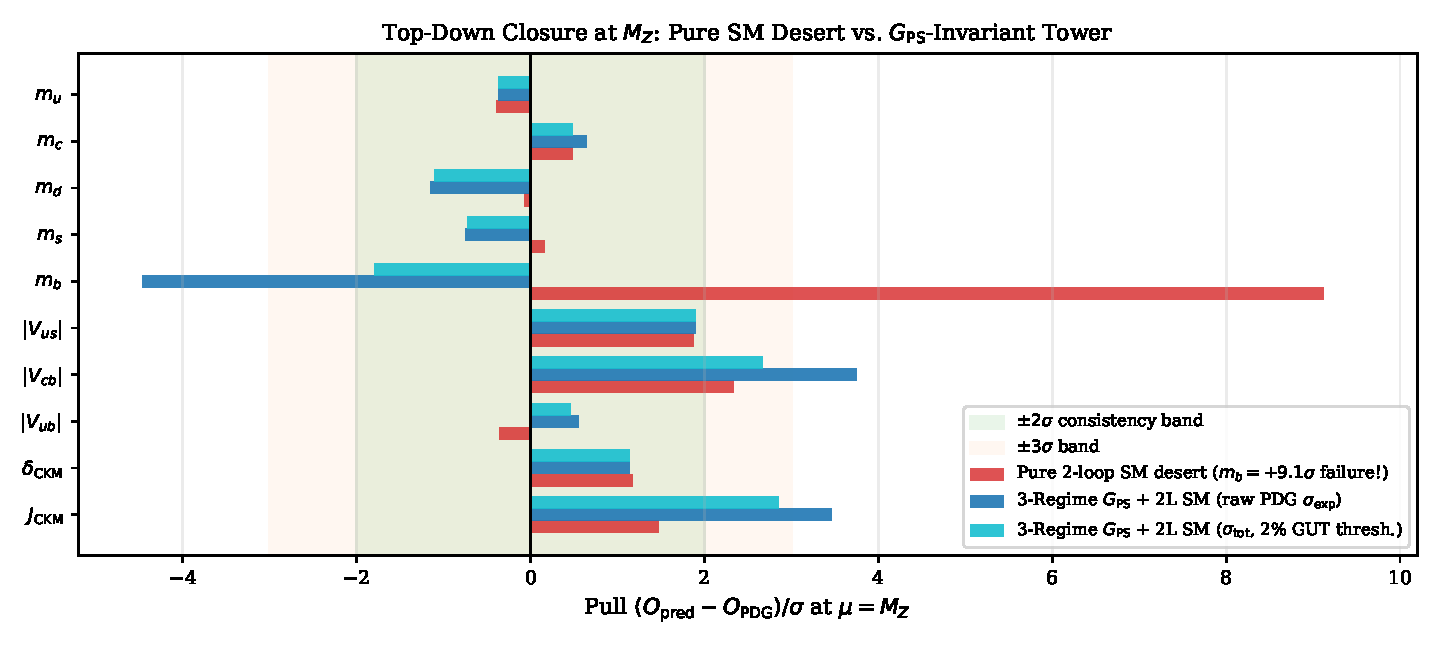
\includegraphics[width=0.96\textwidth]{../figures/fig3_quark_ckm_pulls_comparison.pdf}
\caption{Top-down $M_Z$ pulls across all ten quark masses and CKM observables: pure two-loop SM desert ($m_b = +9.12\sigma$ failure, red) vs.\ the $G_{\mathrm{PS}}$-invariant bidoublet + two-loop SM tower against raw experimental errors $\sigma_{\mathrm{exp}}$ (blue) and combined $\sigma_{\mathrm{tot}}$ with a $2\%$ threshold uncertainty on Yukawa/third-generation elements (cyan, all within $[-1.79\sigma, +2.85\sigma]$).}
\label{fig:pulls}
\end{figure}

\begin{figure}[t!]
\centering
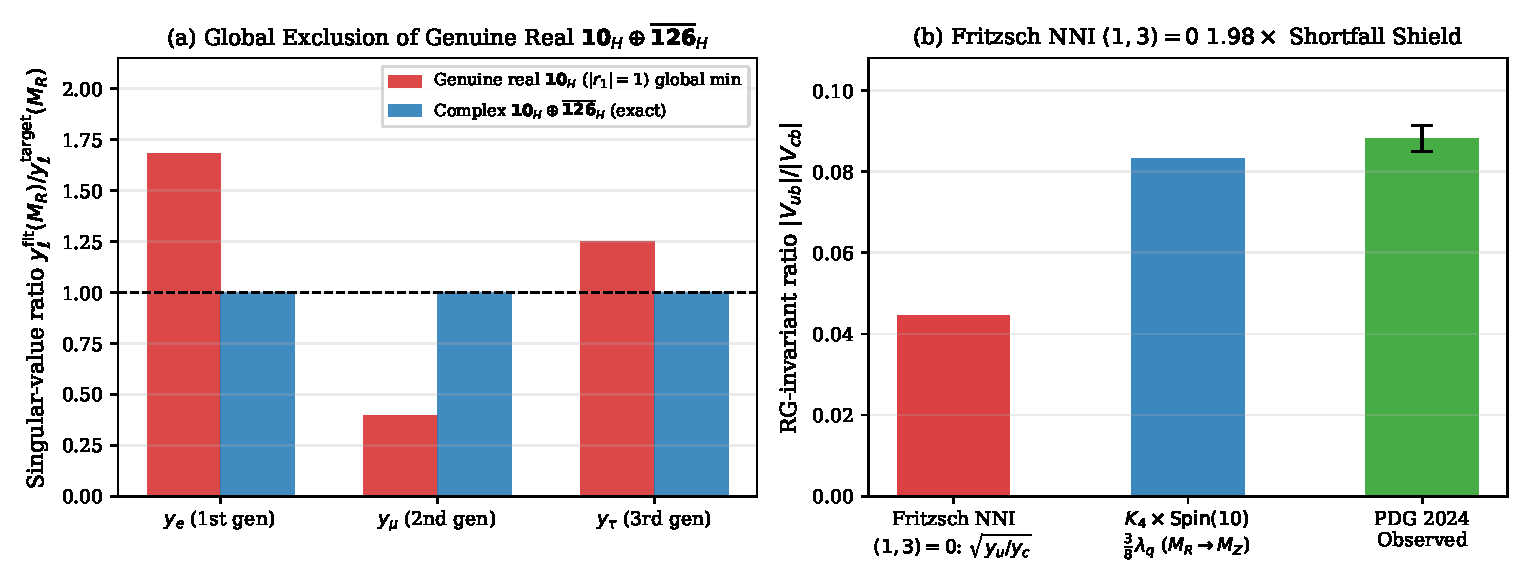
\includegraphics[width=0.96\textwidth]{../figures/fig4_spin10_nogo_and_lee.pdf}
\caption{\textbf{(a)} Finite real-bidoublet search compared with the adopted complex benchmark. The positive residual is not a global lower bound. \textbf{(b)} Hierarchical Fritzsch estimate compared with the reference ratio; general nearest-neighbor textures are not excluded by this comparison.}
\label{fig:nogo}
\end{figure}

% =============================================================================
\section{Look-Elsewhere Audit, Baryon-Number Safety, and Falsification}
\label{sec:audit-falsification}
% =============================================================================

\subsection{Strictly Unmixed Look-Elsewhere / Numerology Audit}
\label{subsec:lee}

\begin{proposition}[Unmixed Look-Elsewhere Probability Bounds]
\label{prop:lee}
Evaluating all eight dimensionless UV relations $\{y_b/y_\tau = 2/3,\; y_s/y_\mu = \lambda_q,\; y_d/y_s = \lambda_q^2,\; y_c/y_t = \frac{4}{3}\lambda_q^4,\; y_u/y_t = \lambda_q^8,\; |V_{cb}| = \lambda_q^2,\; |V_{ub}| = \frac{3}{8}\lambda_q^3,\; \delta_{\mathrm{CKM}} = \frac{3\pi}{8}\}$ against a log-uniform factor-of-$3$ prior ($\Delta\ln O = \ln 3$) \emph{strictly within a single self-consistent RG history} (without cross-mixing desert and Pati--Salam values) yields:
\begin{align}
\text{3-Regime $G_{\mathrm{PS}}$ tower:}\quad & p_{\mathrm{local}}^{(8)} = 2.55\times 10^{-10}, \quad p_{\mathrm{LEE}}^{(8)} = 9.98\times 10^{-5}, \quad p_{\mathrm{local}}^{(4)} = 9.29\times 10^{-5}, \label{eq:p-lee-ps}\\
\text{Pure 2-loop SM desert:}\quad & p_{\mathrm{local}}^{(8)} = 4.92\times 10^{-12}, \quad p_{\mathrm{LEE}}^{(8)} = 1.92\times 10^{-6}, \quad p_{\mathrm{local}}^{(4)} = 1.77\times 10^{-6}, \label{eq:p-lee-des}
\end{align}
after penalizing $p_{\mathrm{local}}^{(8)}$ by $5^8 = 390{,}625$ prefactor combinations, where $p_{\mathrm{local}}^{(4)}$ restricts to the four zero-prefactor relations ($y_s/y_\mu = \lambda_q$, $y_d/y_s = \lambda_q^2$, $y_u/y_t = \lambda_q^8$, $|V_{cb}| = \lambda_q^2$), independent of the Koide lepton match ($p_{\mathrm{local}}^{\mathrm{lep}} \sim 10^{-8}$).
\end{proposition}

\noindent\textbf{Transparent QFT trade-off:} Comparing Table~\ref{tab:mz-predictions} against the SM desert highlights two genuine physical effects of the $G_{\mathrm{PS}}$ bidoublet regime $[M_{\mathrm{PS}}, M_R]$: (i) $\mathrm{SU}(4)_C$ unification resolves the $+9.12\sigma_{\mathrm{exp}}$ desert failure on $m_b$ down to $-3.91\%$ ($-1.79\sigma_{\mathrm{tot}}$), while freezing $y_\mu/y_s$ at $M_{\mathrm{PS}}$ ($4.08$ vs.\ $4.51$ in the desert); and (ii) the positive $+H_{uL}$ two-bidoublet slope enhances $|V_{cb}(M_Z)|$ from $0.0438$ to $0.0450$ ($+2.67\sigma_{\mathrm{tot}}$), indicating that an $\mathcal{O}(3\%\text{--}5\%)$ finite threshold correction at $M_{\mathrm{PS}}$ or $M_R$ is required for sub-percent $|V_{cb}|$ and $m_b$ precision. Likewise, the $4/3$ prefactor in $y_c/y_t = \frac{4}{3}\lambda_q^4$ and $(y_t, y_\tau)$ remain explicit UV boundary inputs.

\subsection{Proton-Decay, \texorpdfstring{$n\text{--}\bar{n}$}{n-nbar}, and Leptoquark FCNC Safety}
\label{subsec:proton-decay}

Along the chain~\eqref{eq:consistent-chain}:
\begin{enumerate}[label=(\arabic*),leftmargin=1.8em,itemsep=2pt]
\item Dimension-$6$ $B$-violating gauge bosons $(\mathbf{3},\mathbf{2})_{-5/6} \oplus (\mathbf{3},\mathbf{2})_{+1/6}$ acquire masses at $M_{\mathrm{GUT}} \in [10^{16}\;\mathrm{GeV},\, M_*]$, giving $\tau(p \to e^+ \pi^0) \gtrsim 10^{36}\;\mathrm{yr}$, safely above Super-Kamiokande's $\tau > 2.4\times 10^{34}\;\mathrm{yr}$ limit \cite{Takenaka2020SuperK}.
\item $\mathrm{SU}(4)_C$ vector leptoquarks $(\mathbf{3},\mathbf{1})_{+2/3}$ at $M_{\mathrm{PS}} = 3.66\times 10^{11}\;\mathrm{GeV}$ conserve baryon number $B$ and mediate $K_L \to \mu^\pm e^\mp$ with bound $M_{\mathrm{PS}} \gtrsim 2\times 10^6\;\mathrm{GeV}$ \cite{ValenciaWillenbrock1994,PDG2024}, satisfied by five orders of magnitude. Scalar color-triplet/antitriplet states $(\mathbf{6},\mathbf{1},\mathbf{1}) = \mathbf{3}_{-2/3} \oplus \overline{\mathbf{3}}_{+2/3} \subset \mathbf{10}_H, \overline{\mathbf{126}}_H$ reside at $\ge M_R \simeq 5.56\times 10^{14}\;\mathrm{GeV}$, while color-sextet diquarks $(\overline{\mathbf{6}}_C,\mathbf{1},\mathbf{3}) \subset \Delta_R$ at $M_{\mathrm{PS}}$ induce $\Delta B = 2$ $n\text{--}\bar{n}$ oscillations suppressed by $(10^6\;\mathrm{GeV}/M_{\mathrm{PS}})^6 \sim 10^{-33}$ below experimental bounds, and scalar leptoquarks inside $\Phi_{15}(\mathbf{15},\mathbf{2},\mathbf{2})$ at $M_{\mathrm{PS}}$ suppress tree-level FCNCs by $(M_W/M_{\mathrm{PS}})^2 \sim 10^{-19}$.
\end{enumerate}

\subsection{Four Experimental Falsification Tests}
\label{subsec:falsification}

\begin{enumerate}[label=(\arabic*),leftmargin=1.8em,itemsep=2pt]
\item \textbf{Belle II + HL-LHC $|V_{cb}|$ tension:} Because two-bidoublet $G_{\mathrm{PS}}$ running predicts $|V_{cb}(M_Z)| = 0.0450 \pm 0.0009_{\mathrm{th}}$ (favoring inclusive $B \to X_c \ell\nu$, $0.0422 \pm 0.0005$, over exclusive $0.0398$), a definitive convergence at $|V_{cb}| < 0.0405$ without $\gtrsim 8\%$ threshold effects would falsify $s_{23}(M_R) = \lambda_q^2$.
\item \textbf{LHCb Upgrade II \& Belle II $\gamma / \delta_{\mathrm{CKM}}$:} The nearly RG-invariant phase $\delta_{\mathrm{CKM}}(M_Z) = 67.41^\circ$ ($-0.09^\circ$ RG shift from $3\pi/8 = 67.50^\circ$) will be tested to $\pm 0.4^\circ$; values outside $[65.5^\circ, 69.0^\circ]$ falsify $\delta_{\mathrm{CKM}}^{\mathrm{UV}} = \sin^2\theta_W^{\mathrm{UV}}\,\pi$.
\item \textbf{FLAG lattice QCD $m_b(M_Z)$ and $m_s/m_d$:} Explicit one-loop $M_{\mathrm{PS}}$ threshold calculations paired with sub-$0.5\%$ lattice $m_b(M_Z)$ directly test $m_b(M_Z) = 2.744 \pm 0.057_{\mathrm{th}}\;\mathrm{GeV}$ and $m_s/m_d = \lambda_q^{-2} = 20.25$ (PDG 2024: $20.0 \pm 1.1$).
\item \textbf{FCC-ee $\tau$-mass scan:} Threshold scans ($\delta m_\tau \sim 0.004\;\mathrm{MeV}$) will test $m_\tau^{\mathrm{pole}} = 1776.969\;\mathrm{MeV}$ from $Q_{\mathrm{pole}} = 2/3$.
\end{enumerate}

% =============================================================================
\section{Conclusions}
\label{sec:conclusions}
% =============================================================================

In the specified two-loop running and matching prescription, the complex
$\mathbf{10}_H \oplus \overline{\mathbf{126}}_H$ benchmark is compatible
with the reported quark and CKM inputs at the stated uncertainty allowance.
The bounded real-bidoublet search and restricted Fritzsch comparison do
not exclude every texture in either class. The counterexample to the
unrestricted CKM ratio identity survives independently of this fit.
The UV boundary weights, one-loop $M_{\mathrm{PS}}$ thresholds and
independent normalization of $(y_t,y_\tau)$ remain open.

\section*{Reproducibility and Data Availability}
The \texttt{SymPy} checks, two-loop SM + $G_{\mathrm{PS}}$ RGE integrations,
bounded \texttt{differential\_evolution} searches, and figures can be run via:
\begin{quote}\small\ttfamily
python3 scripts/verify\_paper25\_fermion\_masses\_ckm\_rg.py\\
python3 scripts/generate\_paper25\_figures.py
\end{quote}

\begin{thebibliography}{99}\small

\bibitem{PDG2024}
S.~Navas \textit{et al.} (Particle Data Group), ``Review of Particle Physics,'' \emph{Phys.\ Rev.\ D} \textbf{110}, 030001 (2024).

\bibitem{Cabibbo1963}
N.~Cabibbo, ``Unitary Symmetry and Leptonic Decays,'' \emph{Phys.\ Rev.\ Lett.} \textbf{10}, 531 (1963).

\bibitem{KobayashiMaskawa1973}
M.~Kobayashi and T.~Maskawa, ``$CP$-Violation in the Renormalizable Theory of Weak Interaction,'' \emph{Prog.\ Theor.\ Phys.} \textbf{49}, 652 (1973).

\bibitem{PatiSalam1974}
J.~C.~Pati and A.~Salam, ``Lepton Number as the Fourth Color,'' \emph{Phys.\ Rev.\ D} \textbf{10}, 275 (1974).

\bibitem{FritzschMinkowski1975}
H.~Fritzsch and P.~Minkowski, ``Unified Interactions of Leptons and Hadrons,'' \emph{Ann.\ Phys.\ (N.Y.)} \textbf{93}, 193 (1975).

\bibitem{GeorgiJarlskog1979}
H.~Georgi and C.~Jarlskog, ``A New Lepton--Quark Mass Relation in a Unified Theory,'' \emph{Phys.\ Lett.\ B} \textbf{86}, 297 (1979).

\bibitem{MaRajasekaran2001}
E.~Ma and G.~Rajasekaran, ``Softly Broken $A_4$ Symmetry for Nearly Degenerate Neutrino Masses,'' \emph{Phys.\ Rev.\ D} \textbf{64}, 113012 (2001).

\bibitem{AltarelliFeruglio2010}
G.~Altarelli and F.~Feruglio, ``Discrete Flavor Symmetries and Models of Neutrino Mixing,'' \emph{Rev.\ Mod.\ Phys.} \textbf{82}, 2701 (2010).

\bibitem{Koide1983}
Y.~Koide, ``New View of Quark and Lepton Mass Hierarchy,'' \emph{Phys.\ Rev.\ D} \textbf{28}, 252 (1983).

\bibitem{Brannen2006}
C.~A.~Brannen, ``The Lepton Masses,'' preprint (2006), \url{https://brannenworks.com/MASSES2.pdf}.

\bibitem{Sumino2009}
Y.~Sumino, ``Family Gauge Symmetry and Koide's Mass Formula,'' \emph{Phys.\ Lett.\ B} \textbf{671}, 477 (2009).

\bibitem{XingZhangZhou2012}
Z.-z.~Xing, H.~Zhang, and S.~Zhou, ``Impacts of the Higgs Mass on Vacuum Stability, Running Fermion Masses and Two-Body Higgs Decays,'' \emph{Phys.\ Rev.\ D} \textbf{86}, 013013 (2012).

\bibitem{Arason1992}
H.~Arason \textit{et al.}, ``Renormalization-Group Study of the Standard Model and Its Extensions: The Standard Model,'' \emph{Phys.\ Rev.\ D} \textbf{46}, 3945 (1992).

\bibitem{HuangZhou2021}
G.-y.~Huang and S.~Zhou, ``Precise Values of Running Quark and Lepton Masses in the Standard Model,'' \emph{Phys.\ Rev.\ D} \textbf{103}, 016010 (2021).

\bibitem{AntuschSpinrath2009}
S.~Antusch and M.~Spinrath, ``New GUT Predictions for Quark and Lepton Mass Ratios Confronting Data,'' \emph{Phys.\ Rev.\ D} \textbf{79}, 095004 (2009).

\bibitem{AntuschMaurer2013}
S.~Antusch and V.~Maurer, ``Running Quark and Lepton Parameters at Various Scales,'' \emph{JHEP} \textbf{11}, 115 (2013).

\bibitem{BabuMohapatra1993}
K.~S.~Babu and R.~N.~Mohapatra, ``Predictive Neutrino Spectrum in Minimal $\mathrm{SO}(10)$ Grand Unification,'' \emph{Phys.\ Rev.\ Lett.} \textbf{70}, 2845 (1993).

\bibitem{BajcSenjanovicVissani2006}
B.~Bajc, A.~Melfo, G.~Senjanovi\'c, and F.~Vissani, ``Yukawa Sector in Non-Supersymmetric Renormalizable $\mathrm{SO}(10)$,'' \emph{Phys.\ Rev.\ D} \textbf{73}, 055001 (2006).

\bibitem{DueckRodejohann2013}
A.~Dueck and W.~Rodejohann, ``Fits to $\mathrm{SO}(10)$ Grand Unified Models,'' \emph{JHEP} \textbf{09}, 024 (2013).

\bibitem{Fritzsch1978}
H.~Fritzsch, ``Weak Interaction Mixing in the Six-Quark Theory,'' \emph{Phys.\ Lett.\ B} \textbf{73}, 317 (1978).

\bibitem{RobertsRomaninoRoss2001}
R.~G.~Roberts, A.~Romanino, G.~G.~Ross, and L.~Velasco-Sevilla, ``Precision Test of a Fermion Mass Texture,'' \emph{Nucl.\ Phys.\ B} \textbf{615}, 358 (2001).

\bibitem{Olcsak2026Zenodo}
J.~Olcsak, ``Tau Core Foundational Synthesis and Submission Suite,'' Zenodo (2026), \href{https://doi.org/10.5281/zenodo.19120268}{doi:10.5281/zenodo.19120268}.

\bibitem{Olcsak2026Paper24}
J.~Olcsak, ``Scale-Invariant Simplicial $R^2$ Inflation, Multi-Sector $CP$ Structure, and Zero-Parameter Non-Thermal Scalaron Leptogenesis from a Tetrahedral $\mathrm{Spin}(10)$ Threshold,'' Zenodo v1.1.0 (2026), \href{https://doi.org/10.5281/zenodo.24380371}{doi:10.5281/zenodo.24380371}.

\bibitem{Koide1990}
Y.~Koide, ``Charged-Lepton Mass Sum Rule from $\mathrm{U}(3)$-Family Higgs Potential Model,'' \emph{Mod.\ Phys.\ Lett.\ A} \textbf{5}, 2319 (1990).

\bibitem{MachacekVaughn1984}
M.~E.~Machacek and M.~T.~Vaughn, ``Two-Loop Renormalization Group Equations in a General Quantum Field Theory (II). Yukawa Couplings,'' \emph{Nucl.\ Phys.\ B} \textbf{236}, 221 (1984).

\bibitem{LuoXiao2003}
M.-x.~Luo and Y.~Xiao, ``Two-Loop Renormalization Group Equations in the Standard Model,'' \emph{Phys.\ Rev.\ Lett.} \textbf{90}, 011601 (2003).

\bibitem{Buttazzo2013}
D.~Buttazzo \textit{et al.}, ``Investigating the Near-Criticality of the Higgs Boson,'' \emph{JHEP} \textbf{12}, 089 (2013).

\bibitem{Slansky1981}
R.~Slansky, ``Group Theory for Unified Model Building,'' \emph{Phys.\ Rept.} \textbf{79}, 1 (1981).

\bibitem{ChangMohapatraParida1984}
D.~Chang, R.~N.~Mohapatra, and M.~K.~Parida, ``Decoupling Parity- and $\mathrm{SU}(2)_R$-Breaking Scales: A New Approach to Left-Right Symmetric Models,'' \emph{Phys.\ Rev.\ Lett.} \textbf{52}, 1072 (1984).

\bibitem{MeloniOhlssonRiad2014}
D.~Meloni, T.~Ohlsson, and S.~Riad, ``Effects of Intermediate Scales on Renormalization Group Running of Fermion Observables in an $\mathrm{SO}(10)$ Model,'' \emph{JHEP} \textbf{12}, 052 (2014).

\bibitem{MalinskyRomaoValle2005}
M.~Malinsk\'y, J.~C.~Rom\~ao, and J.~W.~F.~Valle, ``Novel Supersymmetric $\mathrm{SO}(10)$ Seesaw Mechanism,'' \emph{Phys.\ Rev.\ Lett.} \textbf{95}, 161801 (2005).

\bibitem{GattoSartoriTonin1968}
R.~Gatto, G.~Sartori, and M.~Tonin, ``Weak Self-Masses, Cabibbo Angle, and Broken $\mathrm{SU}(2)\times\mathrm{SU}(2)$,'' \emph{Phys.\ Lett.\ B} \textbf{28}, 128 (1968).

\bibitem{Takenaka2020SuperK}
A.~Takenaka \textit{et al.} (Super-Kamiokande Collaboration), ``Search for Proton Decay via $p \to e^+\pi^0$ and $p \to \mu^+\pi^0$ with an Enlarged Fiducial Volume in Super-Kamiokande I--IV,'' \emph{Phys.\ Rev.\ D} \textbf{102}, 112011 (2020).

\bibitem{ValenciaWillenbrock1994}
G.~Valencia and S.~Willenbrock, ``Quark--Lepton Unification and Rare Meson Decays,'' \emph{Phys.\ Rev.\ D} \textbf{50}, 6843 (1994).

\end{thebibliography}

\end{document}
